

\let\negmedspace\undefined
\let\negthickspace\undefined

\documentclass[journal,12pt,twocolumn]{IEEEtran}

%\documentclass[conference]{IEEEtran}
%\IEEEoverridecommandlockouts
% The preceding line is only needed to identify funding in the first footnote. If that is unneeded, please comment it out.
\usepackage{cite}
\usepackage{amsmath,amssymb,amsfonts,amsthm}
\usepackage{algorithmic}
\usepackage{graphicx}
\usepackage{textcomp}
\usepackage{xcolor}
\usepackage{txfonts}
\usepackage{listings}
\usepackage{enumitem}
\usepackage{mathtools}
\usepackage{gensymb}
\usepackage[breaklinks=true]{hyperref}
\usepackage{tkz-euclide} % loads  TikZ and tkz-base
\usepackage{listings}
\usepackage{graphicx}
\usepackage{caption} 
                                          
\DeclareMathOperator*{\Res}{Res}
%\renewcommand{\baselinestretch}{2}
\renewcommand\thesection{\arabic{section}}
\renewcommand\thesubsection{\thesection.\arabic{subsection}}
\renewcommand\thesubsubsection{\thesubsection.\arabic{subsubsection}}

\renewcommand\thesectiondis{\arabic{section}}
\renewcommand\thesubsectiondis{\thesectiondis.\arabic{subsection}}
\renewcommand\thesubsubsectiondis{\thesubsectiondis.\arabic{subsubsection}}

% correct bad hyphenation here
\hyphenation{op-tical net-works semi-conduc-tor}
\def\inputGnumericTable{}                                 %%

\lstset{
%language=C,
frame=single, 
breaklines=true,
columns=fullflexible
}

\begin{document}
%

\newtheorem{theorem}{Theorem}[section]
\newtheorem{problem}{Problem}
\newtheorem{proposition}{Proposition}[section]
\newtheorem{lemma}{Lemma}[section]
\newtheorem{corollary}[theorem]{Corollary}
\newtheorem{example}{Example}[section]
\newtheorem{definition}[problem]{Definition}

%\newcommand{\BEQA}{\begin{eqnarray}}
%\newcommand{\EEQA}{\end{eqnarray}}
%\newcommand{\define}{\stackrel{\triangle}{=}}

\bibliographystyle{IEEEtran}


\newcommand{\define}{\stackrel{\triangle}{=}}
\newcommand{\permcomb}[4][0mu]{{{}^{#3}\mkern#1#2_{#4}}}
\newcommand{\comb}[1][-1mu]{\permcomb[#1]{C}}

%\bibliographystyle{ieeetr}

\providecommand{\mbf}{\mathbf}
\providecommand{\pr}[1]{\ensuremath{\Pr\left(#1\right)}}
\providecommand{\qfunc}[1]{\ensuremath{Q\left(#1\right)}}
\providecommand{\sbrak}[1]{\ensuremath{{}\left[#1\right]}}
\providecommand{\lsbrak}[1]{\ensuremath{{}\left[#1\right.}}
\providecommand{\rsbrak}[1]{\ensuremath{{}\left.#1\right]}}
\providecommand{\brak}[1]{\ensuremath{\left(#1\right)}}
\providecommand{\lbrak}[1]{\ensuremath{\left(#1\right.}}
\providecommand{\rbrak}[1]{\ensuremath{\left.#1\right)}}
\providecommand{\cbrak}[1]{\ensuremath{\left\{#1\right\}}}
\providecommand{\lcbrak}[1]{\ensuremath{\left\{#1\right.}}
\providecommand{\rcbrak}[1]{\ensuremath{\left.#1\right\}}}
\theoremstyle{remark}
\newtheorem{rem}{Remark}
\newcommand{\sgn}{\mathop{\mathrm{sgn}}}
\providecommand{\abs}[1]{\left\vert#1\right\vert}
\providecommand{\res}[1]{\Res\displaylimits_{#1}} 
\providecommand{\norm}[1]{\left\lVert#1\right\rVert}
%\providecommand{\norm}[1]{\lVert#1\rVert}
\providecommand{\mtx}[1]{\mathbf{#1}}
\providecommand{\mean}[1]{E\left[ #1 \right]}
\providecommand{\fourier}{\overset{\mathcal{F}}{ \rightleftharpoons}}
%\providecommand{\hilbert}{\overset{\mathcal{H}}{ \rightleftharpoons}}
\providecommand{\system}{\overset{\mathcal{H}}{ \longleftrightarrow}}
	%\newcommand{\solution}[2]{\textbf{Solution:}{#1}}
\newcommand{\solution}{\noindent \textbf{Solution: }}
\newcommand{\cosec}{\,\text{cosec}\,}
\providecommand{\dec}[2]{\ensuremath{\overset{#1}{\underset{#2}{\gtrless}}}}
\newcommand{\myvec}[1]{\ensuremath{\begin{pmatrix}#1\end{pmatrix}}}
\newcommand{\mydet}[1]{\ensuremath{\begin{vmatrix}#1\end{vmatrix}}}

\let\vec\mathbf


\vspace{3cm}

\title{
\textbf{Hardware Asssignment Report}\\Random Number Generation using Shift Registers
}

\author{CS22BTECH11046\\P.Yasaswini}	
 




\maketitle

\newpage

%\tableofcontents

\bigskip

\renewcommand{\thefigure}{\theenumi}
\renewcommand{\thetable}{\theenumi}



\textbf{COMPONENTS}. 
\begin{table}[htbp]
\centering

\begin{tabular}{|c|c|c|}
\hline
\textbf{Components } & \textbf{Value} & \textbf{Quantity} \\
\hline
Breadboard & & 1 \\
\hline
Seven Segment Display& Common Anode & 1\\
\hline
Decoder & 7447& 1\\
\hline
Flip Flop & 7474& 2\\
\hline
X-OR GATE &7486 & 1\\
\hline
555 IC& & 1\\
\hline
Resistor& 1K$\Omega$ & 1\\
\hline
Resistor &1M$\Omega$  & 1\\
\hline
Capacitor &100nF & 1\\
\hline
Capacitor & 10nF& 1\\
\hline
Jumper Wires & & 3\\
\hline
\end{tabular}



\caption{}
\end{table}

\textbf{DESCRIPTION}.
\begin{enumerate}
\item Giving power supply to Breadboard through connecting USB to micro USB board and give  VCC(+5V) power supply and ground the respective rails in breadboard.
\item Generated clock using 555 timer by using two capacitors (10nF,100nF) , one resistor 1M$\Omega$ and jumper wires.It will the convert regular pulse into Square pulse.
\item Made a circuit using one Decoder(7447) used to covert binary input into specific output pattern, one X-OR gate(7486) and two D-Flip flops(7474) used to store a single bit of information.
\item Connected the Clock output of 555 timer circuit to Clock signal of D-Flip flops.
\item And make connections between the seven segment display and decoder.
A seven segment display is a electronic display that can show numerical digits (0-9) and some additional characters.
\end{enumerate}
\newpage
\textbf{BLOCK DIAGRAM}.
\begin{figure}[htbp]
\centering
\includegraphics[height=4cm]{block.jpeg}
\captionsetup{justification=centering}
\caption{Block Diagram}
\end{figure}

\textbf{Observation}.
\begin{figure}[htbp]
\centering
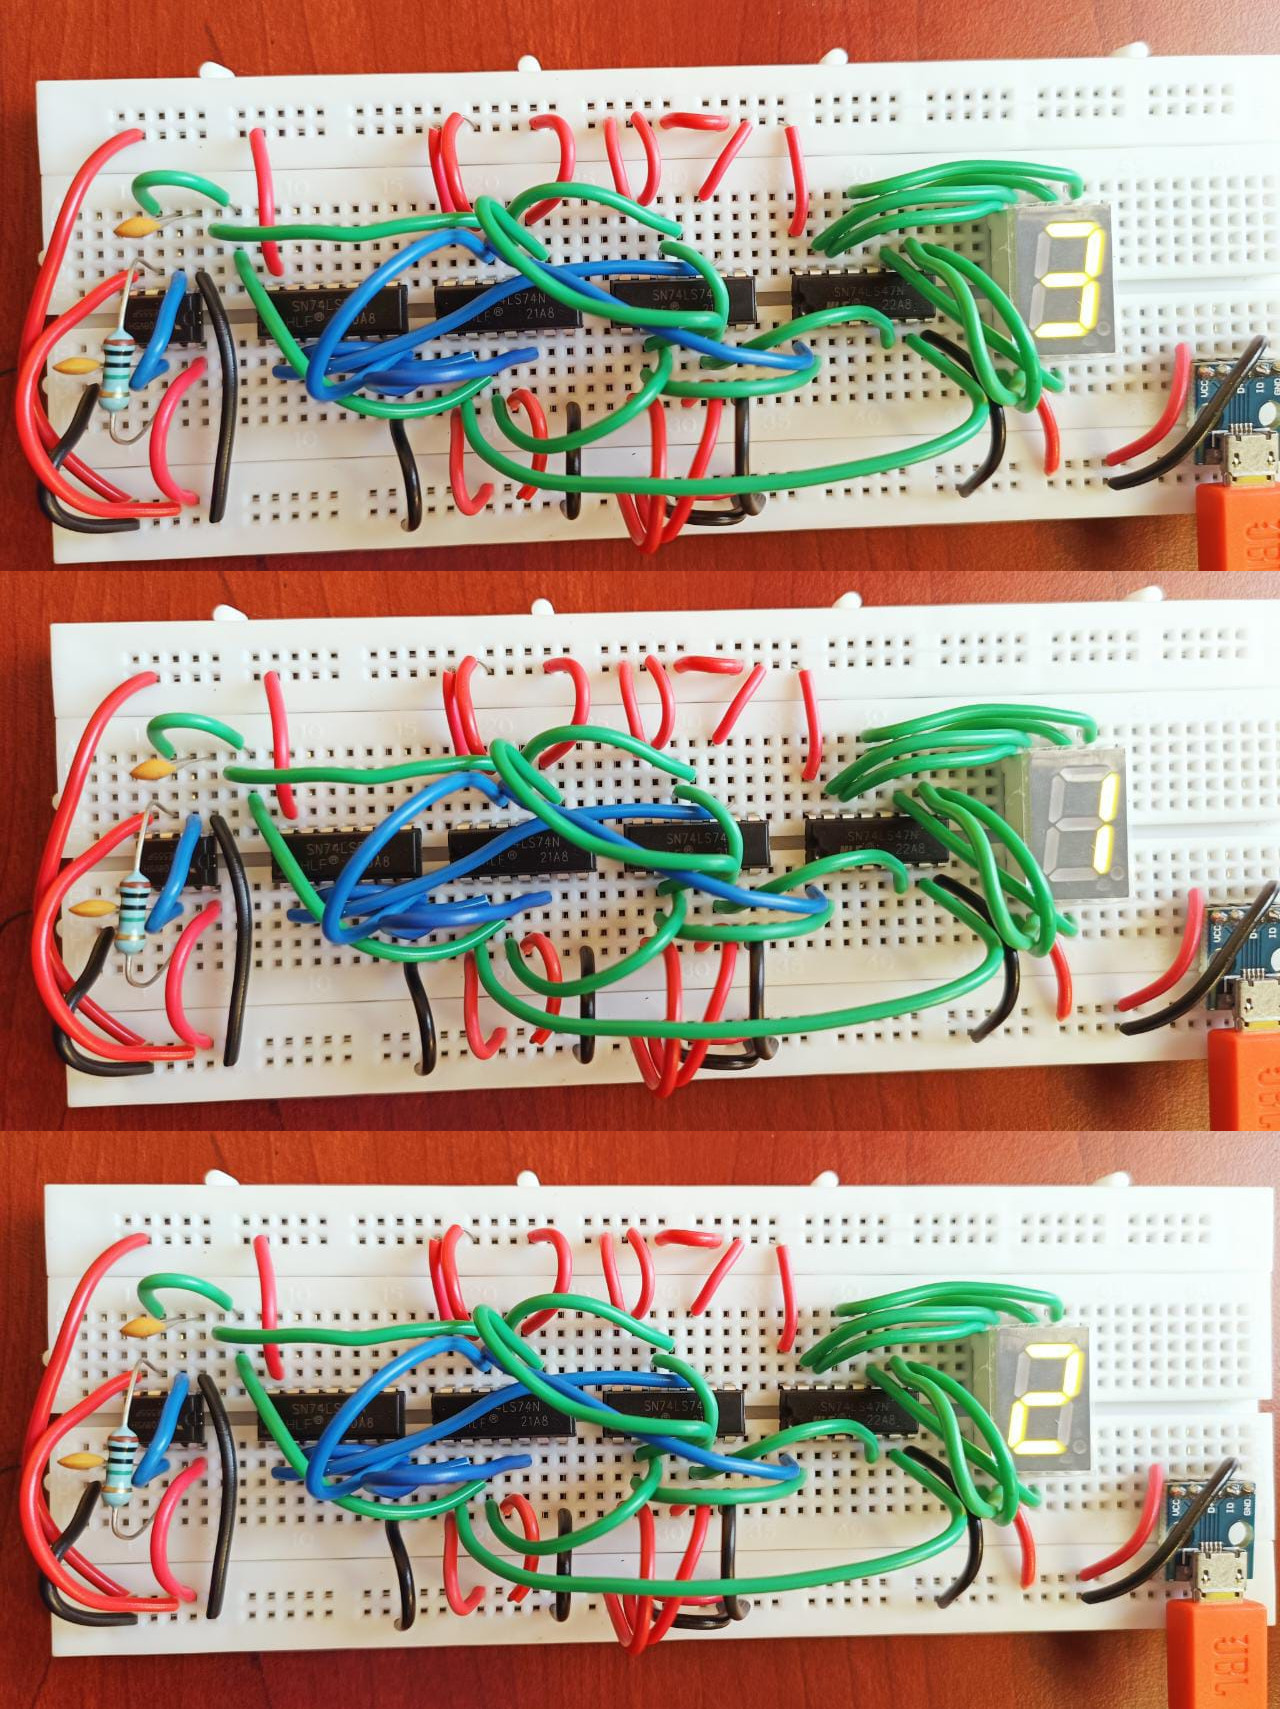
\includegraphics[scale=0.1]{img.jpg}
\captionsetup{justification=centering}
\caption{OBSERVATIONS}
\end{figure}

Random Variables are observed in a A seven segment display, it is showing random numbers between (0-9) and some additional characters

\end{document}


